\boldchapter{The Effect of Endogenous Transcription on Origin Specification} \label{repRes}


In chapter \ref{replicationIntro}, I discussed the mechanisms of DNA replication and how extrinsic factors, such as chromatin structure, can affect origin efficiency. Despite many years of study, the effect of transcription on the activity of replication origins remains a controversial topic, as evidence exists for both a negative and a positive role. 
Here we show that physiological levels of transcription have a negative impact on origin activity and that mechanisms exist to limit the interference between transcription and replication initiation.

In this work I applied metagene analyses to several published datasets in order to obtain a global view of polymerase occupancy and termination events around origins. I then used correlative techniques to explore the relationships between transcription levels and different stages of replication initiation. Nothern blot analyses were performed by Julien Gros in the lab. Preliminary data regarding origin efficiency in Nrd1 defective strains (see discussion, section \ref{repDisc}) was generated by our collaborator Julien Soudet, I performed the computational analyses. 

\singlespacing
\section{Global Visualization of Transcription Around Replication Origins}
\doublespacing

In order to have a global view of transcription around replication origins, we decided to produce aggregate plots using published polymerase occupancy datasets \cite{schaughency:2014:genomewide} around sites of replication initiation. This powerful technique allows to visualize average transcription levels at a single nucleotide resolution across any number of genomic loci, but requires a common feature along which all loci can be aligned (e.g. an annotated feature or a sequence element, such as a TSS or a transcription factor binding site). Because of the nature of replication origins, we chose the ACS—the only sequence element absolutely required for origin activity—as our common feature. 

\begin{figure}[ht]

\centering
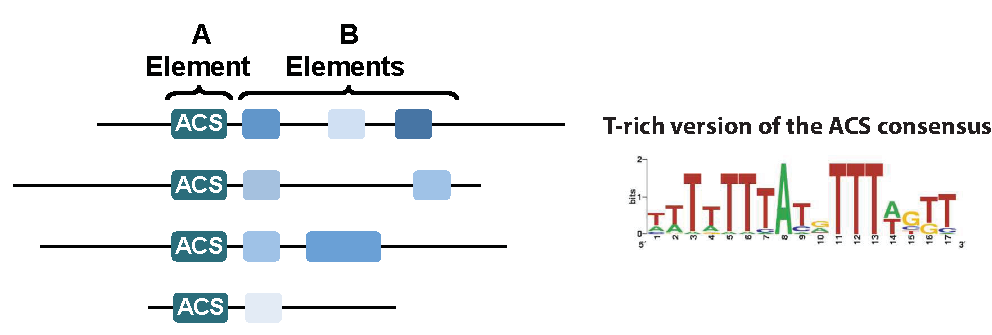
\includegraphics[width=\textwidth]{figures/results/acs}
\caption[ACS consensus and arrangement relative to other origin DNA elements]{Cartoon showing the most typical arrangement of sequence elements within origins. the ACS is required, while several B elements contribute to origin specification dowstream of the T-rich strand of the ACS.}
\label{fig:originSchema}

\end{figure}

The ACS is an AT-rich sequence element that is bound by the ORC complex and acts as the assembly site for the pre-replication complex. Because of its non-palindromic sequence, we could appropriately distinguish between transcription along the T-rich or A-rich versions of the ACS consensus. Additionally, the orientation of the ACS determines the location of other important sequence elements of the origin, the B elements (Fig. \ref{fig:originSchema}). This allowed us to not only be strand-specific with respect to the ACS, but with respect to the whole structure of the origin. 

\singlespacing
\section{Transcriptional Pausing and Termination Are Associated With Replication Origins}
\doublespacing

The meta-site analysis of RNAPII occupancy around replication origins is shown in figure \ref{fig:metagenes}A. The top part of the plot represents transcription along the T-rich strand of the ACS, while the bottom part represents transcription along the A-rich strand of the ACS. To obtain this plot, we used a set of origins for which the ACS was annotated \cite{nieduszynski:2006:genomewide}. Because transcription in origins is generally low, we restricted our analysis to those surrounded by convergent or tandem genes in order to have a more distinct signal. 



We detect an increase in polymerase occupancy, relative to the incoming average, in the vicinity of the ACS for both along the T- and A-rich strands of the ACS.
However, while transcription on the T-rich strand shows a distinct occupancy peak about 20-30 nucleotides before the ACS, transcription on the A-rich strand displays multiple peaks that reside 110-130 nucleotides away from it.
 Additionally, both occupancy increases—especially the one of the T-rich strand—are characterized by a steep drop in signal after their peak. Because of this sharp drop, we reasoned that the peaks could represent polymerase pausing caused by transcription termination. 
We therefore generated an aggregate plot across all origins, showing the location of termination events (as defined by the production of RNA 3’-ends \cite{wilkening:2013:efficient}) relative to the position of the ACS (fig \ref{fig:metagenes}B). 
We detected a substantial number of termination events in the vicinity of the ACS. 
Moreover, the asymmetry that we highlighted between the two strands with respect to polymerase occupancy is maintained in this analysis. 
The peak of termination events in the T-rich strand resides about 20 nucleotides from the ACS, while in the A-rich strand this peak is shifted ~100 nucleotides away from the ACS. 
\begin{figure}[hp!]

\centering
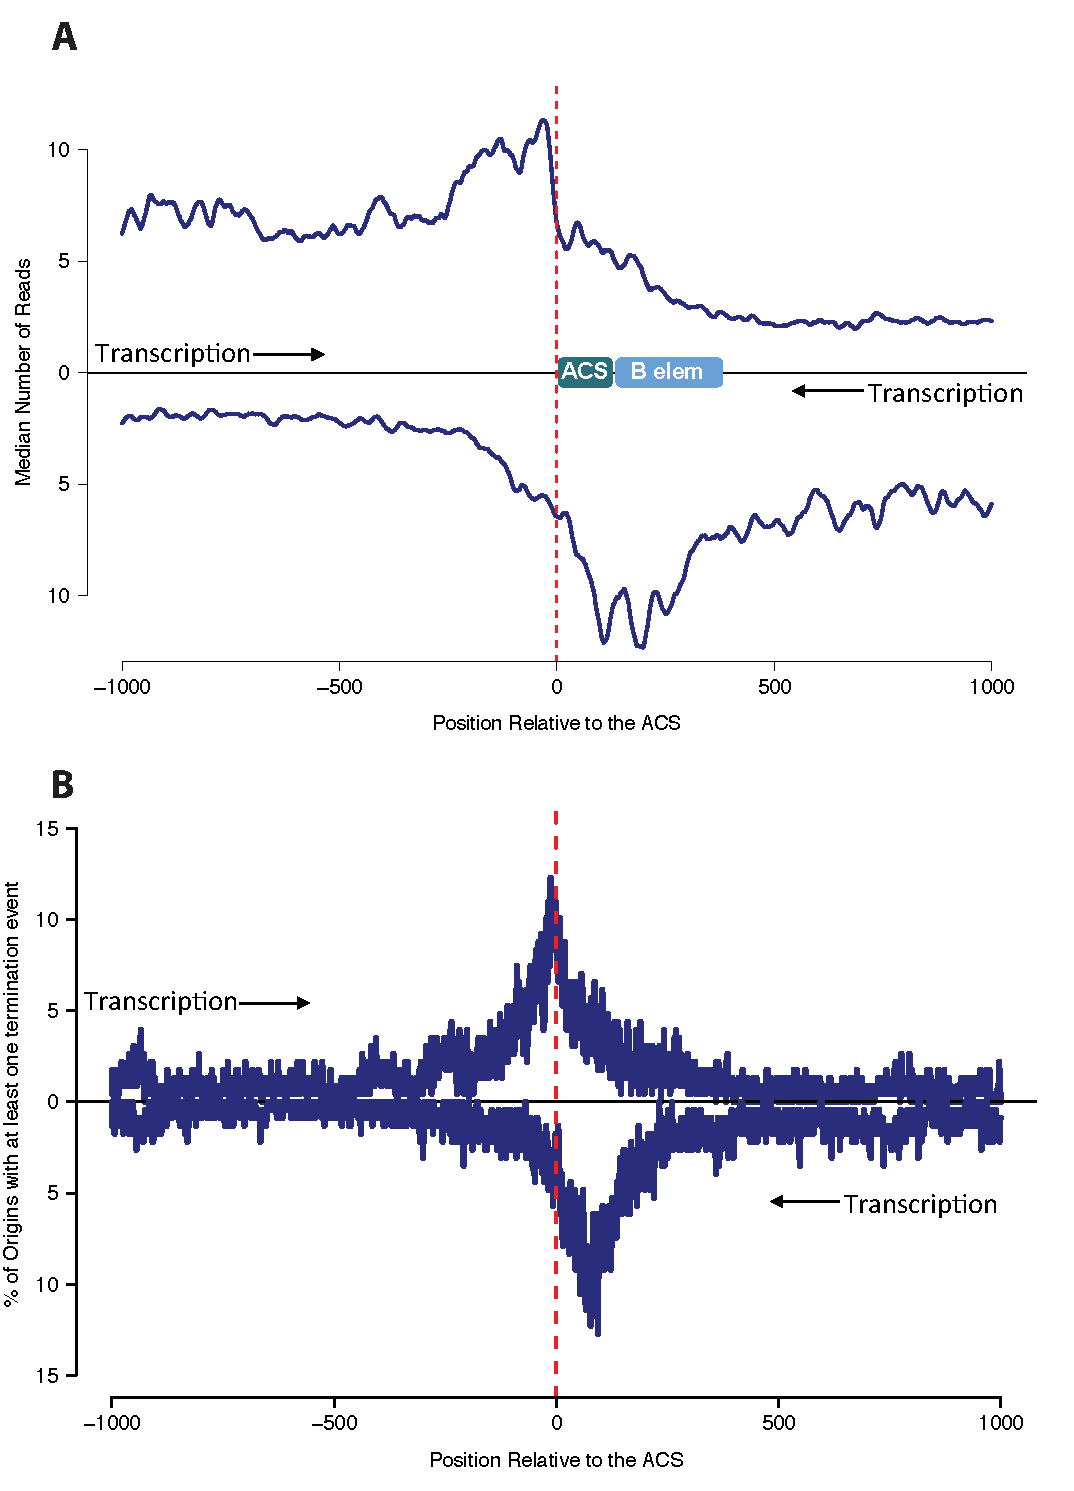
\includegraphics[width=0.95\textwidth]{figures/results/metagenes}
\caption[Metagene analyses showing polymerase occupancy and termination around replication origins]{\textbf{A: }Metagene analysis performed on a polymerase occupancy dataset \cite{schaughency:2014:genomewide}. profiles represent the average levels of transcription across origins surrounded by convergent and tandem genes. The top part of the plot represents transcription along the T-rich strand of the ACS, while the bottom part represents transcription along the A-rich strand of the acs. \textbf{B: } Plot representing the percentage of assayed origins with at least one termination event at any given position. }
\label{fig:metagenes}

\end{figure}  
These results show that RNAPII accumulates around replication origins, and this accumulation coincides with transcription termination events. 
  
Although we did not know which pathway was responsible for the termination events we detected around origins, we identified several hallmarks of road-block termination. Polymerase pausing is coincident with precise termination and, at least in the case of the T-rich strand, is positioned ~20 nucleotides before the binding site of a DNA binding factor. This led us to speculate that termination on the T-rich strand is caused by a road-block dependent on ORC. 

\begin{figure}[h]

\centering
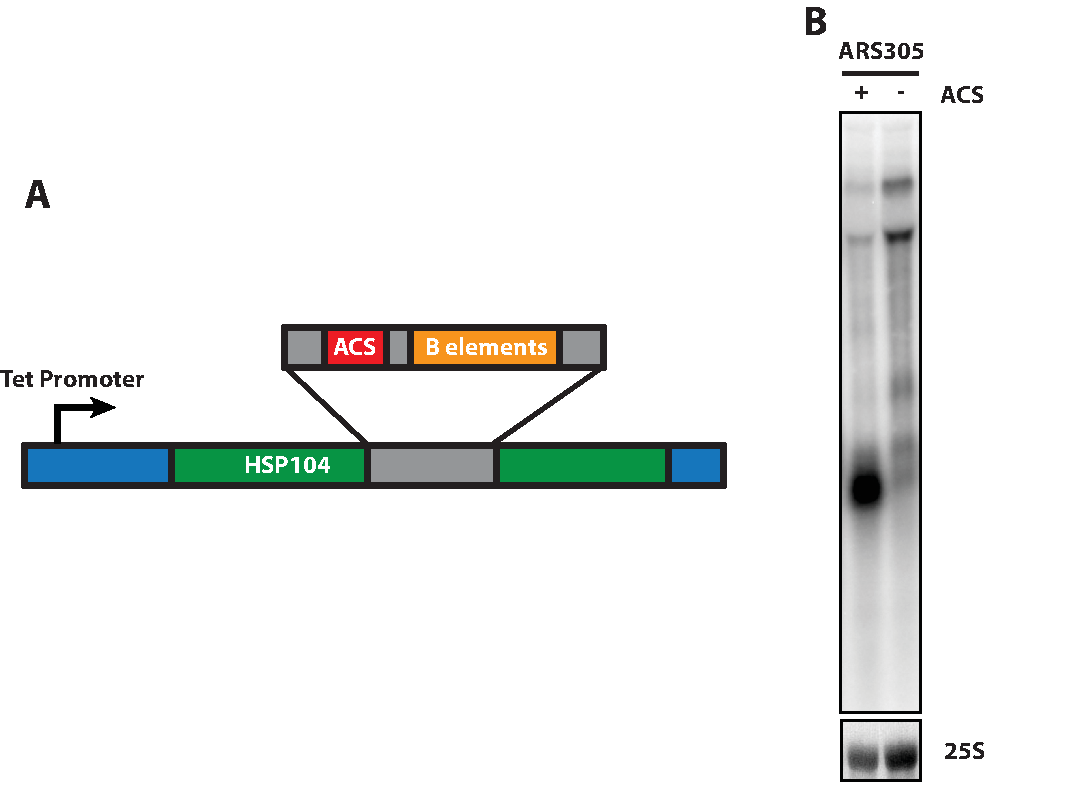
\includegraphics[width=\textwidth]{figures/results/northern}
\caption[Northern blot analysis of transcription through ARS305]{\textbf{A: }In our reporter system, a tet promoter directs transcription of a fragment of the HSP104 gene, whithin which ARS305 is embedded with or without the ACS. \textbf{B: } Northern blot analysis of the reporter system shows the presence of a short transcript that disappear upon ACS deletion. }
\label{fig:northern}

\end{figure}  

In order to test this hypothesis, Julien Gros, post-doc in the lab, performed northern blots using a reporter system. In this system, the sequence of interest is embedded in a fragment of the HSP104 gene, whose expression is then driven by a strong promoter (Fig \ref{fig:northern}A). 
We tested the sequence of origin ARS305 carrying the deletion of the ACS sequence. 
Figure \ref{fig:northern}B shows species generated by transcription through the T-rich strand of the ACS in presence or absence of the ACS sequence itself. 
Strong signal for a short transcript is detectable when the ACS is present, while in its absence, the short transcript disappears to the profit of a longer species. 
Although we cannot formally exclude that sequence elements are playing a role in transcription termination of the short species, this results argues in favor of termination by a road-block mechanism.

\singlespacing
\section{Transcription Levels Asymmetrically Affect Origin Efficiency}
\doublespacing

Road-block is known to act as fail-safe termination to protect promoter regions and other loci from transcriptional interference \cite{colin:2014:roadblock}. 
We reasoned that termination enacted by ORC could have a similar role by protecting the B elements, which are known to aid in pre-RC assembly \cite{wilmes:2002:b2}. 
\begin{figure}[h]

\centering
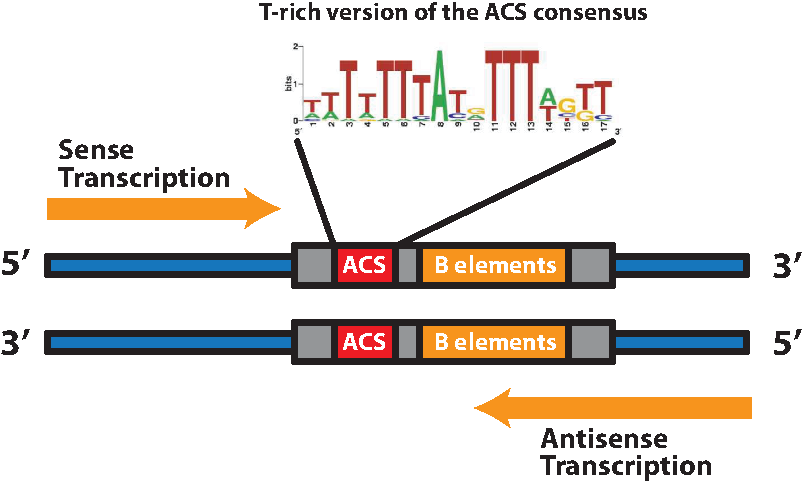
\includegraphics[width=\textwidth]{figures/results/senseAntisenseSchema}
\caption[Cartoon of sense and antisense transcription relative to the ACS]{Schematic representation of ``sense" and ``antisense" transcription relative to the structure of the origin. While sense transcription can be blocked by ORC before reaching the B elements, antisense transcription has no such impairments.}
\label{fig:senseAntisense}

\end{figure}  
Because of the arrangement of ACS and B elements within origins, however, ORC would only be able to block transcription coming along the T-rich strand of the ACS before the B elements are invaded. To test this hypothesis, we therefore correlated several measures of origin efficiency with levels of transcription upstream of the ACS on both its T-rich and A-rich strands. 
In order to obtain these values, we calculated the average polymerase occupancy in a 100 nucleotide window upstream of the ACS. Transcription levels calculated along the T-rich strand of the ACS were dubbed ``sense", while transcription levels calculated over the A-rich strand of the ACS were dubbed ``antisense" (figure \ref{fig:senseAntisense}).



As replication occurs in discrete steps, we wanted to know if either sense or antisense transcription were affecting any particular stage of replication initiation. We therefore correlated per-origin estimates of licensing efficiency, firing efficiency, and timing of firing \cite{hawkins:2013:highresolution} with our estimates of sense and antisense transcription. Our approach was two-fold: for every measure of origin efficiency, we calculated the Pearson’s correlation between it and the levels of sense and antisense transcription. In parallel, we obtained two subpopulations of origins, according to either transcription or efficiency, and compared them using boxplots and t-tests for statistical significance.

\subsection{Licensing Efficiency}

Licensing is the first step in DNA replication, however, not all origins are licensed during the cell cycle.
Every origin we considered is associated with a value between zero and one, representing the likelihood that the origin will be licensed during the cell cycle \cite{hawkins:2013:highresolution}. 
We split the population of origins into two sub-populations according to high and low transcription for both sense and antisense. 
We then compared the distribution of licensing efficiencies in these two sub-populations. 
Analysis of the overall populations showed no difference in licencing efficiency whether origins are surrounded by high or low sense or antisense transcription (Fig. \ref{fig:licensing}A). 
A statistically significant anti-correlation between antisense transcription levels and licensing efficiency (pearson’s $r$ = -0.15 with $p$ = 0.03) could be observed, but no significant correlation between sense transcription levels and licensing efficiency (pearson’s $r$ = -0.04 with $p$ = 0.53). 
\begin{figure}[hp!]

\centering
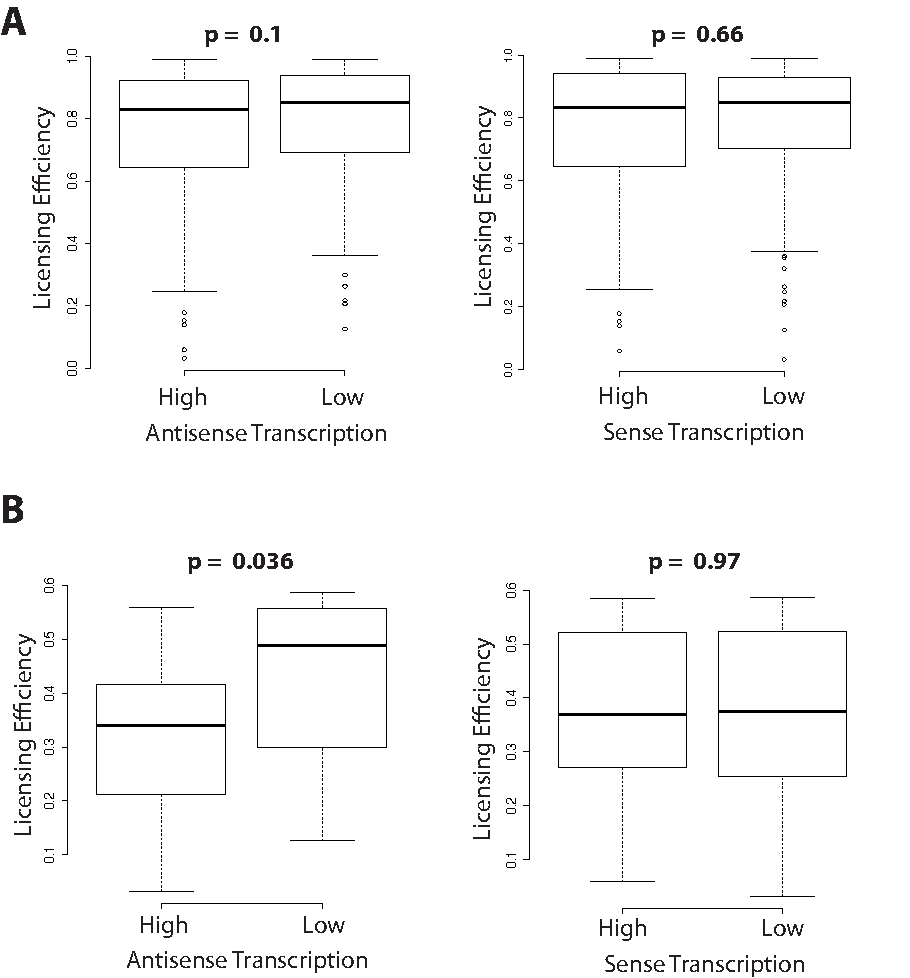
\includegraphics[width=\textwidth]{figures/results/competence}
\caption[Boxplots comparing licensing efficiencies in high- and low-transcription populations]{These boxplots compare the distribution of licensing efficiencies between high- and low-transcription populations.\textbf{A: }Boxplots generated using the totality of the origins available to us. high- and low-transcription populations show similar levels of efficiency both according to sense and antisense transcription. \textbf{B: } In this experiment, we restricted our boxplots to poorly licensed origins. Higher levels of antisense transcription are now significantly associated with lower efficiency, while high or low sense transcription displays no difference. }
\label{fig:licensing}

\end{figure} 
We reasoned that the low levels of endogenous transcription might not be sufficient to affect highly efficient origins. We therefore considered only origins with relatively low licensing efficiency ($<$ 0.6) and repeated the experiment (fig \ref{fig:licensing}B). 
A significant difference in the distribution of licensing efficiencies could be detected between populations with high and low antisense transcription. 
However, no such a difference could be detected when the two populations were chosen according to sense transcription. 
These results are supported by the Pearson’s correlation coefficients: the anti-correlation between antisense transcription and licensing efficiency is higher (pearson’s $r$ = -0.32 with $p$ = 0.04), while that between sense transcription and licensing efficiency remains low (pearson’s $r$ = 0.03 with $p$ = 0.83). 
Taken together, these results support the notion that physiological levels of transcription antisense to the ACS can negatively affect licensing origins, while sense transcription—regardless of its intensity—does not affect significantly licensing efficiency.



\subsection{Firing Efficiency}

Firing is the process that allows licensed origins to activate and begin the replicative process. This step is conditional on the presence of the pre-replication complex, and therefore cannot occur unless the origin has been previously licensed. To define classes of origins with different firing efficiencies, we compared licensing and firing for every origin using published data. As for licencing, the probability of firing has been defined by a value between zero and one \cite{hawkins:2013:highresolution}.

\begin{figure}[h!]

\centering
\includegraphics[width=\textwidth]{figures/results/firing}
\caption[Boxplots comparing transcription levels in high- and low-firing populations]{These boxplots compare the distribution of sense an antisense transcription levels between populations with high and low firing efficiency. \textbf{A: }Plot of licensing efficiency vs firing efficiency. Because firing requires licensing, similar efficiency values in these two metrics denote highly efficiently firing origins. We therefore consider those origins close to the diagonal as efficient origins and those below as inefficient. \textbf{B: } Boxplots comparing the distribution of sense and antisense transcription levels between origins with low and high firing efficiency. The population with low firing efficiency are significantly associated with higher antisense transcription levels, but this relationship does not hold in the case of sense transcription. }
\label{fig:firing}

\end{figure} 

A scatterplot of firing and licensing efficiencies is represented in fig \ref{fig:firing}A.
We divided origins into two populations according to their position in this plot.
Origins residing around the diagonal are able to fire efficiently, as licensing and firing have similar likelihoods and firing requires licensing. Origins residing below the diagonal, however, fire inefficiently, as their firing efficiency is lower than their licensing efficiency. 
In figure \ref{fig:firing}B we compare the distribution of antisense and sense transcription levels between these two populations. Inefficiently firing origins display higher levels of antisense transcription relative to efficiently firing origins, however, this relationship is lost when considering sense transcription. 
These results are supported by Pearson’s correlations: antisense transcription is anti-correlated with normalized firing efficiencies (pearson’s $r$ = -0.18 with $p$ = 0.01) while sense transcription and normalized firing efficiencies do not seem to be correlated (pearson’s $r$ = 0.06 with $p$ = 0.39). 
Taken together, these results suggest that not only licensing, but also firing is affected by antisense transcription levels, while sense transcription levels have no effect on this step.


\subsection{Timing of Firing}

While firing efficiency is a measure of how often a particular origin is able to initiate DNA replication, it does not give information about the elapsed time between the entry in S-phase and activation of the replisome. 
We wanted to assess whether transcription levels influence the timing of origin firing. 
In figure \ref{fig:timing} we compare the distribution of median firing times for high and low, sense and antisense transcription. 
High antisense transcription is significantly associated with higher median replication times, while no difference in median replication times can be detected between high or low sense transcription levels. 
\begin{figure}[h!]

\centering
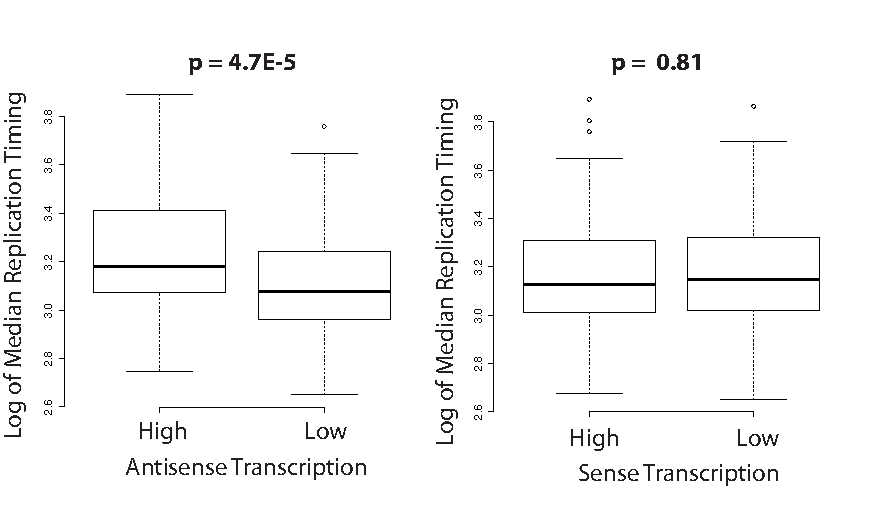
\includegraphics[width=0.97\textwidth]{figures/results/timing}
\caption[Boxplots comparing median replication times in high- and low-transcription populations]{These boxplots represent the distribution of median replication times in population with high, low, sense, and antisense transcription. High antisense transcription correlates with higher replication times relative to low antisense transcription. However, sense high and low sense transcription seems to have no effect on replication timing.}
\label{fig:timing}

\end{figure} 
These results are also supported by correlations that do not rely on subpopulations: antisense transcription levels positively correlate with median replication times (pearson’s $r$ = 0.19 with $p$ = 0.008) while sense transcription levels show no correlation (pearson’s $r$ = -0.05 with $p$ = 0.42). These results suggest that even when firing occurs, antisense transcription levels can delay firing, possibly by interfering with the assembly of the replisome, while sense transcription levels have no impact.

\clearpage

\section{Discussion} \label{repDisc}

In this work, we investigated the relationship between the process of origin specification and that of RNA transcription. We analyzed transcription around replication origins separately on both strands and detected localized increases in polymerase occupancy that coincided with hotspots of transcription termination. We noticed that pausing and termination were arranged asymmetrically relatively to the ACS, with a major peak immediately upstream of the ACS in the T-rich orientation (position -25) of and several peaks indicating accumulation of polymerases at different distances (-100 to -125) upstream of the ACS in the  A-rich  orientation.

We explored the possibility that ORC binding to the ACS might induce road-block termination at these sites through northern blot analysis of ARS305. This experiment revealed that transcription upstream of the ACS in the T-rich strand orientation is terminated in an ACS-dependent manner. Experiments were also performed to assess the occurrence of termination for transcription entering the ACS from the opposite direction (upstream of the A-rich strand) but the results were not conclusive because a site of NNS-dependent termination was present that masked the possible ACS-dependent termination. At this stage we do not know whether the additional peaks of polymerase pausing at position -100 to -125 upstream of the ACS in the A-rich strand orientation are due to roadblocked polymerases or polymerases paused for other reasons.  

However, prompted by the asymmetry revealed by these experiments, we tested the hypothesis that transcription levels could asymmetrically impact origin efficiency depending on origin orientation. We correlated per-origin estimates of licensing efficiency, firing efficiency, and timing of firing with surrounding transcription levels both sense and antisense relative to origins oriented by the T-rich strand of the ACS. High levels of transcription on the antisense strand proved to negatively impact every measure of replication efficiency, while sense transcription had no significant effect.

\singlespacing
\subsection{Transcription Termination Is a Feature of Replication Origins}
\doublespacing

Our meta-site analyses provided insights on the global state of polymerase occupancy and transcription termination around replication origins genome-wide. According to this global view, many origins are associated with distinct peaks of polymerase pausing and transcription termination on both sense and antisense strands. Because of the complexity of the DNA replication process, as well as previous evidence emerging from the literature, we speculate that these termination events protect the origin by preventing transcriptional interference. In accordance with this model, we have evidence that transcription on the sense strand of the ACS is terminated by ORC through road-block, a mechanism already known to protect promoter regions from invading polymerases. This model is supported by preliminary analyses of polymerase occupancy datasets generated in strains defective for either CPF or NNS termination. Both datasets displayed a marked increase in polymerase pausing in the vicinity of ORC, a phenotype consistent with the increased readthrough transcription that is stalled at the site of road-block. While the meta-site analyses provided many elements that suggested road-block by ORC, we could not formally prove that its presence is responsible for the termination. In our case study, ARS305, we show that termination is ACS dependent, but cannot exclude that sequence elements within the ACS could be the determinant for termination. 

\singlespacing
\subsection{ACS Orientation Determines the Impact of Transcription on Replication Efficiency}
\doublespacing

In order to explore the impact of endogenous transcription on DNA replication, we decided to correlate strand specific transcription levels with measures of origin efficiency. Through these analyses we showed that high levels of transcription generally correlate with poor replication performance, however, only transcription entering the origin from upstream of the A-rich strand of the ACS displays such correlations. We propose a model whereby a road-block enacted by ORC is sufficient to prevent endogenous levels of RNAPII from elongating into the B elements, thus preventing transcription from interfering with the replicative process (Fig. \ref{fig:model}). Transcription on the other strand, however, might be terminated less efficiently which might not be sufficient to prevent all incoming polymerases from invading the B elements and affecting one or more DNA replication steps. 

\begin{figure}[h]

\centering
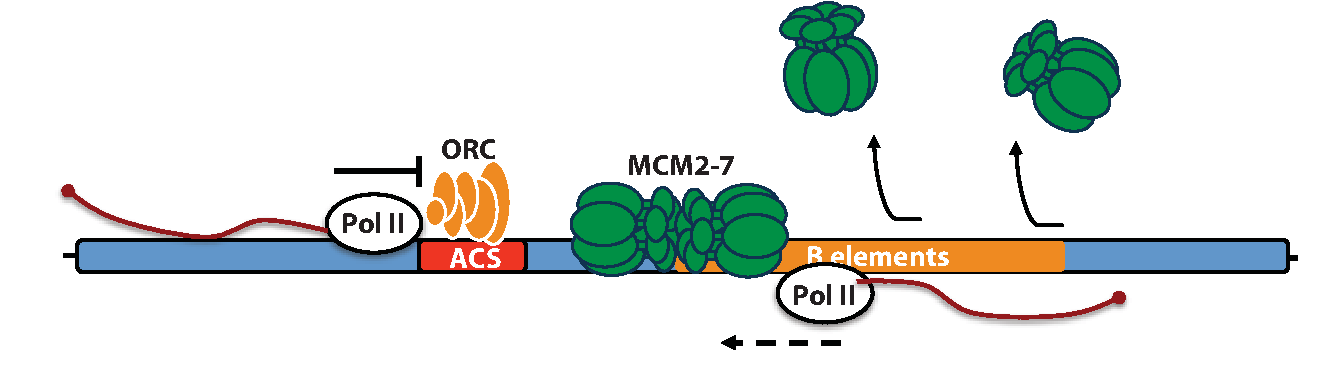
\includegraphics[width=\textwidth]{figures/results/model}
\caption[A model of how transcription can affect replication efficiency]{Model of how transcription can asymmetrically affect replication efficiency. While sense transcription can be efficiently blocked by the ACS before reaching the B elements, antisense transcription can invade the B elements more efficiently.}
\label{fig:model}

\end{figure} 

Julien Soudet, one of our collaborators, generated some preliminary data measuring replication efficiency in a strain defective for NNS termination. We calculated Pearson’s correlation between antisense transcription levels and replicative efficiency relative to wild type. A strong anticorrelation between the two quantities was observed (Fig. \ref{fig:JS}), implying that stronger antisense transcription relative to wild type is associated with reduced replication activity. Surprisingly, correlation between relative sense transcription levels and relative replicative efficiency also displays a negative trend (Fig.  \ref{fig:JS}), albeit lower than in the antisense case. These results suggest that the increased transcription resulting from defects in NNS termination are enough to overcome the road-block and generate defects in replication efficiency independent of the orientation of the origin. however, they also suggest that transcription termination on the sense strand is likely stronger than that on the antisense strand, as it is less associated with poor replicative performance. 

\begin{figure}[h]

\centering
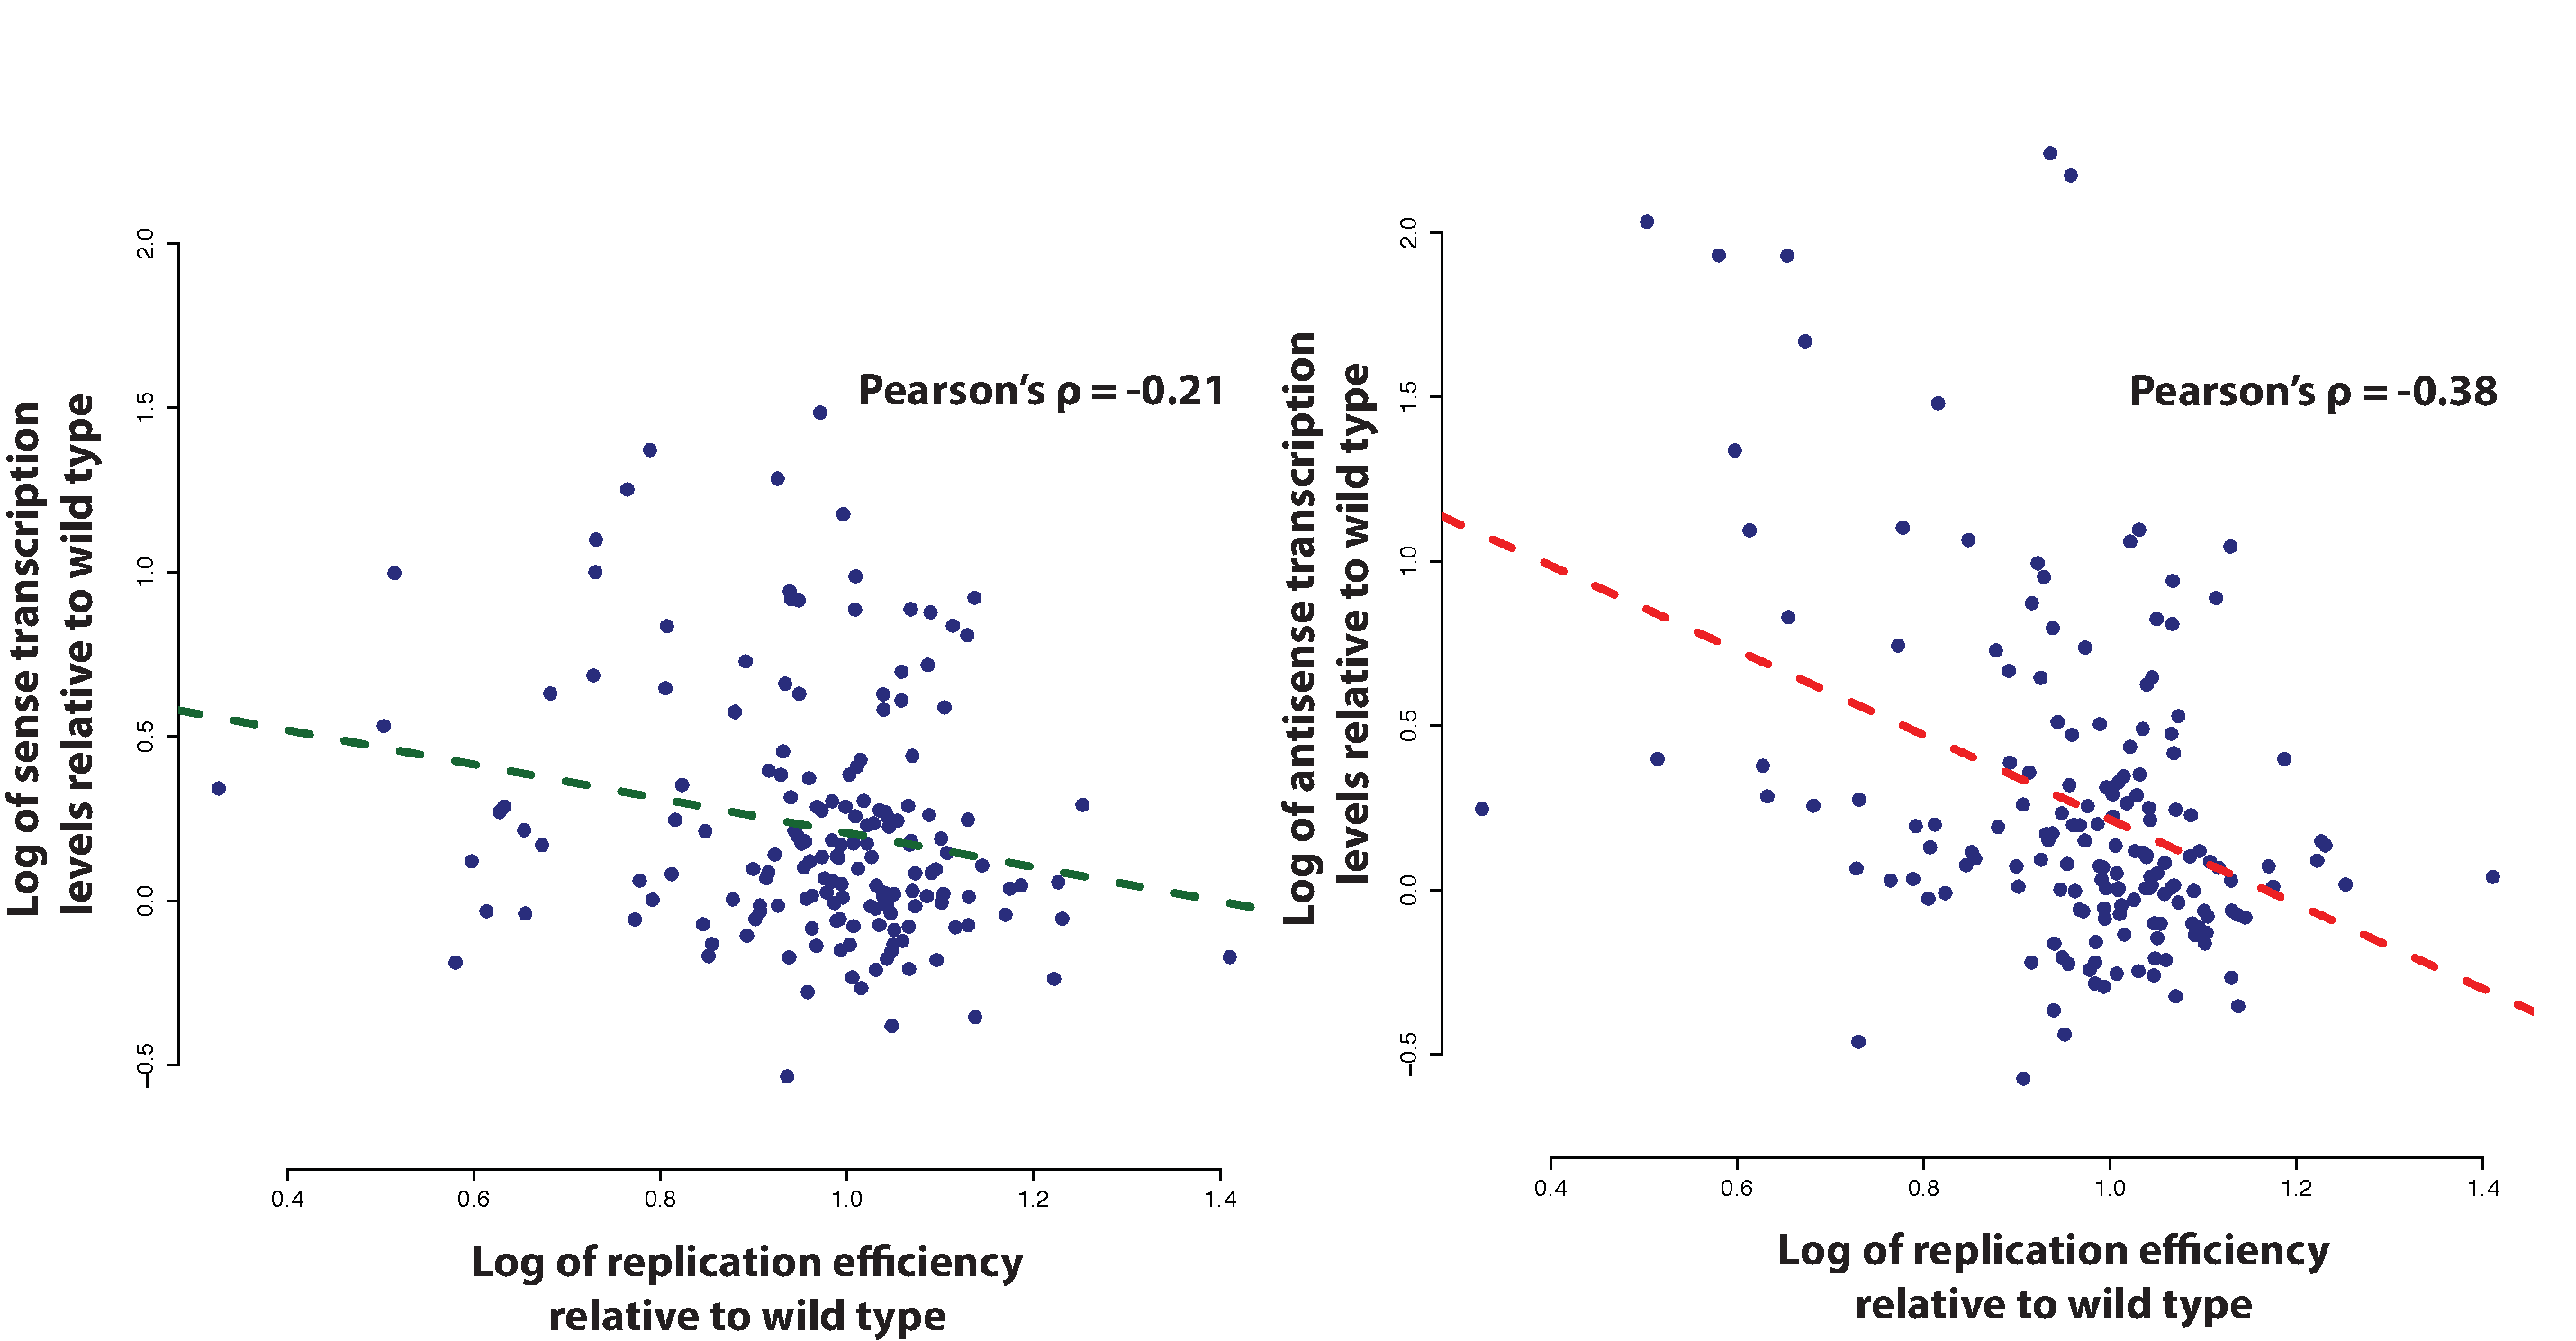
\includegraphics[width=\textwidth]{figures/results/JScorrelations}
\caption[Correlations between transcription and replication efficiency in a NNS defective strain]{Scatterplots of relative sense and antisense transcription levels versus relative replication efficiencies. Each axis displays the log$_2$ ratio between levels of transcription or replication efficiency in a NNS-defective strain relative to wild type. In this non-physiological condition, both sense and antisense transcription levels anticorrelate with replication efficiency. However, antisense transcription levels remain more strongly associated with poor replicative efficiency.}
\label{fig:JS}

\end{figure} 


Overall, downregulation of replicative activity seems to be a function of the quantity of polymerases that transcribes through the core sequence elements of the origin. 
However, it is difficult to assess the mechanistic reasons for this phenotype. 
Transcription might directly displace or otherwise interfere with elements of the pre-RC. 
Alternatively, it is tempting to speculate that transcription-dependent nucleosome deposition might interfere with assembly or firing of the replication complex.

\clearpage
